
\section{Red konvergence}

Zanima nas ali lahko povemo kaj o redu konvergence. Izkaže se, da lahko za nekatere (pogoste) primere dokažemo, da je red konvergence vsaj kvadratičen. Za ta dokaz najprej potrebujemo dve pomožni lemi.

\begin{lema}\label{prvalema}
Naj bo ${\bf f}$ ravninska B\`{e}zierjeva krivulja in ${\bf p}$ njena optimalna $L_2$ aproksimacija stopnje $k$. Potem obstaja konstanta $C$, da za poljuben interval $[\alpha,\beta]\subseteq[0,1]$ velja $\lVert {\bf f} - {\bf p} \rVert _{BB}^{[\alpha,\beta]} \leq C |\alpha - \beta|^{k+1}$.
\end{lema}
\proof
Spomnimo se, da za poljubni normi $\lVert\, \cdot\, \rVert _1$ in $\lVert\, \cdot \,\rVert _2$ na končno dimenzionalnem vektorskem prostoru $V$ obstajata konstanti $0 < C_1 \leq C_2$, tako da je 
\begin{equation}\label{norm_equiv}
C_1 \lVert v\rVert _2 \leq \lVert v\rVert _1 \leq C_2 \lVert v\rVert _2, \; v\in V.
\end{equation}
Zato obstajata konstanti $D_1$ in $D_2$, da je $\lVert {\bf r}\rVert _{BB}^{[\alpha,\beta]} \leq D_1 \lVert {\bf r}\rVert _2^{[\alpha,\beta]}$ in $\lVert {\bf r}\rVert _{2}^{[\alpha,\beta]} \leq D_2 \lVert {\bf r}\rVert _\infty^{[\alpha,\beta]}$ za vsak ${\bf r}\in  \Pi _{[\alpha,\beta]}^n$. Pri tem konstanti $D_1$ in $D_2$ nista odvisni od intervala $[\alpha,\beta]$, saj so norme invariantne glede afine transformacije domene.

Od tod sledi, da je 
$\lVert {\bf f} - {\bf p} \rVert _{BB}^{[\alpha,\beta]} \leq D_1 \lVert {\bf f} - {\bf p} \rVert _{2}^{[\alpha,\beta]}$. Naj bodo komponente ${\bf q}_\alpha$ Taylorjevi polinomi stopnje $k$ razviti okrog točke $t = \alpha$ za vsako komponento krivulje ${\bf f}$. Potem velja
$$
D_1 \lVert {\bf f} - {\bf p} \rVert _{2}^{[\alpha,\beta]} \leq D_1 \lVert {\bf f} - {\bf q}_\alpha \rVert _{2}^{[\alpha,\beta]},
$$
saj je ${\bf p}$ optimalna $L_2$ aproksimacija za ${\bf f}$. Iz \ref{norm_equiv} sledi, da je 
$
D_1 \lVert {\bf f} - {\bf q}_\alpha \rVert _{2}^{[\alpha,\beta]} \leq D_1D_2 \lVert {\bf f} - {\bf q}_\alpha \rVert _{\infty}^{[\alpha,\beta]}
$. Spomnimo se, da lahko razliko med ${\bf f}(t) - {\bf q}_\alpha(t)$ zapišemo v obliki
$$
{\bf f}(t) - {\bf q}_\alpha(t) = \frac{{\bf f}^{(k+1)}(t_o)}{(k+1)!}(t-\alpha)^{k+1},
$$
kjer je ${\bf f}^{(k+1)}$ $(k+1)$-vi odvod krivulje ${\bf f}$ in kjer vse člene opazujemo po komponentah. Od tod dobimo oceno
$$
D_1D_2 \lVert {\bf f} - {\bf q}_\alpha \rVert _{\infty}^{[\alpha,\beta]} \leq
\frac{\sqrt{2}}{(k+1)!}D_1D_2\max _{t\in [0,1]} \lVert {\bf f}^{(k+1)}(t_0) \rVert |\alpha - \beta|^{k+1}.
$$
\endproof

\begin{lema}\label{drugalema}
Naj bo ${\bf f}$ ravninska B\`{e}zierjeva krivulja stopnje $n$. Potem obstajajo konstante $C_{j}$, tako da za poljuben interval $[\alpha,\beta]\subseteq[0,1]$ in optimalno $L_2$ aproksimacijo ${\bf p}$ stopnje $k$ od ${\bf f}$ velja
$\lVert {\bf f}^{(j)} - {\bf p}^{(j)} \rVert _{\infty} \leq C_{j}|\alpha - \beta|^{k+1-j}$, za $j=0,1,\ldots,k$. 
\end{lema}
\proof
Definirajmo novo normo s predpisom
$$
\lVert {\bf r}\rVert _{*}^{[\alpha,\beta]} = \lVert {\bf r}\rVert _\infty^{[\alpha,\beta]} + |\alpha - \beta|\lVert {\bf r}'\rVert _\infty^{[\alpha,\beta]} + \ldots + 
 |\alpha - \beta|^k\lVert {\bf r}^{(k)}\rVert _\infty^{[\alpha,\beta]}.
$$
To je res norma, saj je $\lVert \,\cdot\, \rVert _\infty$ norma. Zaradi invariance norm pod afino transformacijo obstaja konstanta $D_1$, ki je neodvisna od intervala $[\alpha,\beta]$, tako da je 
$$
\lVert {\bf r}\rVert _{*}^{[\alpha,\beta]} \leq D_1 \lVert {\bf r}\rVert _{2}^{[\alpha,\beta]}.
$$
Po eni strani je
\begin{equation}\label{lema2:en1}
\begin{split}
\lVert {\bf f} - {\bf p}\rVert _{*}^{[\alpha,\beta]}  =  \lVert {\bf f} - {\bf p}\rVert _\infty^{[\alpha,\beta]}  &+  |\alpha - \beta|\lVert {\bf f}' - {\bf p}'\rVert _\infty^{[\alpha,\beta]} + \ldots +\\ 
   & +  |\alpha - \beta|^k\lVert {\bf f}^{(k)} - {\bf p}^{(k)}\rVert _\infty^{[\alpha,\beta]} \leq 
 D_1 \lVert {\bf f} - {\bf p}\rVert _{2}^{[\alpha,\beta]},
 \end{split}
\end{equation}
po drugi strani lahko (podobno kot v lemi \ref{prvalema}) s pomočjo Taylorjevega polinoma in izreka o ostanku ocenimo
\begin{equation}\label{lema2:en2}
\begin{split}
D_1 \lVert {\bf f} - {\bf p}\rVert _{2}^{[\alpha,\beta]} \leq 
D_1 \lVert {\bf f} - {\bf q}_\alpha\rVert _{2}^{[\alpha,\beta]} \leq 
D_1D_2 \lVert {\bf f} - &{\bf q}_\alpha\rVert _{\infty}^{[\alpha,\beta]} \leq \\
\frac{\sqrt{2}}{(k+1)!}  D_1D_2\max _{t\in [0,1]}& \lVert {\bf f}^{(k+1)}(t_0) \rVert |\alpha - \beta|^{k+1}.
\end{split}
\end{equation}
\endproof
Iz \ref{lema2:en1} in \ref{lema2:en2} sledijo ocene iz leme.
\begin{definicija}
%\in
%\in \Pi _{[\xi,\eta]}^m
Naj bosta ${\bf f}(t)$ in ${\bf g}(s)$ ravninski B\`{e}zierjevi krivulji s presečiščem ${\bf z}_0 = {\bf f}(t_0) = {\bf g}(s_0)$. Presečišče ${\bf z}_0$ imenujemo:
\begin{itemize}
	\setlength\itemsep{0.33em}
\item {\em transverzalno presečišče}, če je ${\bf f}'(t_0)\times {\bf g}'(s_0) \neq {\bf 0}$,
\smallskip
\item {\em tangentno presečišče}, če je ${\bf f}'(t_0)\times {\bf g}'(s_0) = {\bf 0}$ in ${\bf f}'(t_0)\neq {\bf 0}$, ${\bf g}'(s_0)\neq {\bf 0}$, 
\smallskip
\item {\em degenerirano presečišče}, če je ${\bf f}'(t_0) = {\bf 0}$ ali ${\bf g}'(s_0) = {\bf 0}$.
\end{itemize}
\end{definicija}


\begin{trditev}
Naj imata Bezierjevi krivulji ${\bf f}$ in ${\bf g}$ transverzalno presečišče v ${\bf f}(t_0)={\bf g}(s_0)$. Potem obstajajo konstante $C_f, C_f', C_g$ in $C_g'$, da za dovolj velike $i\in \N$ velja
\begin{equation}\label{prva_neenakost}
|\alpha _{i+1} - \beta _{i+1}| \leq C_f |\alpha _{i} - \beta _{i}|^{k+1} + C_g|\xi _{i} - \eta _{i}|^2
\end{equation}
oz.
\begin{equation}\label{druga_neenakost}
|\xi _{i+1} - \eta _{i+1}| \leq C_f' |\alpha _{i} - \beta _{i}|^{2} + C_g'|\xi _{i} - \eta _{i}|^{k+1}.
\end{equation}
\end{trditev}

\proof
Dokazali bomo le neenakost \ref{prva_neenakost}, saj je dokaz za \ref{druga_neenakost} podoben. 

Naj bosta $[\alpha _i,\beta _i]$ in $[\xi _i,\eta _i]$ zaporedji intervalov, ki jih algoritem generira. Oglejmo si kako se algoritem obnaša za velike $i$. Ker se dolžine intervalov v vsakem koraku zmanjšajo vsaj za polovico, je 
\begin{equation*}
\lim _{i\rightarrow \infty} |\alpha _i-\beta _i| = 0 \,\text{ in }\, \lim _{i\rightarrow \infty} |\xi _i - \eta _i| = 0.
\end{equation*}
 Sledi, da ${\bf b}_0{\bf b}_m$ konvergira proti tangenti ${\bf g}'(s_0)$. Zato gre normala ${\bf n}$ na ${\bf b}_0{\bf b}_m$ proti normali ${\bf n}_0$ na ${\bf g}(s_0)$.

Naj bo $\omega = {\bf n}_0\cdot {\bf f}'(t_0)$. Po predpostavki je ${\bf f}'(t_0)\times {\bf g}'(s_0) \neq {\bf 0}$, torej je $\omega \neq 0$.

Oglejmo si situacijo v $i$-tem koraku algoritma, ki jo prikazuje slika \ref{slika1}. Velja 
$$
|\alpha _{i+1}-\beta _{i+1}| = h_{i+1,{\bf f}} \leq L_{i+1} = l_{i+1,1} + l_{i+1,2} + l_{i+1,3}.
$$
Želimo oceniti člene na desni strani neenakosti. Ker je $\frac{\omega}{4} = \frac{d_{max}-d_{min}}{l_{i+1,1}  + l_{i+1,3}}$ je
\begin{equation}\label{lp13}
l_{i+1,1}  + l_{i+1,3} = \frac{4(d_{max} - d_{min})}{\omega}.
\end{equation}
Želimo oceniti še člen $l_{i+1,2}$. V ta namen si najprej oglejmo ali sta funkciji $d_1(t)$ in $d_2(t)$ naraščajoči. Najprej opazimo, da obstaja tak $\epsilon _1>0$, da je za dovolj velike $i$  
\begin{equation}\label{prva_ocena}
|d'(t_0) - \omega| = |{\bf n}\cdot {\bf f}'(t_0) - {\bf n}_0 \cdot {\bf f}'(t_0)| < \frac{\omega}{4},
\end{equation}
ko je $|\xi _i - \eta _i| < \epsilon _1$, saj gre ${\bf n}$ proti ${\bf n}_0$, ko $i\rightarrow\infty$. Obstaja tudi tak $\epsilon _2 > 0$, da je za dovolj velike $i$
\begin{equation}\label{druga_ocena}
\lVert {\bf f}'(t) - {\bf f}'(t_0)\rVert < \frac{\omega}{4},
\end{equation}
ko je $|\alpha _i - \beta _i| < \epsilon _2$ saj je ${\bf f}'$ zvezna. Dalje obstaja tudi tak $\epsilon _3 > 0$, da za dovolj velike $i$ velja
\begin{equation}\label{tretja_ocena}
|d'(t)-d'_1(t)| < \frac{\omega}{4},
\end{equation}
ko je $|\alpha _i - \beta _i| < \epsilon _3$, saj po lemi \ref{drugalema} velja
$$
|d'(t)-d'_1(t)| = |{\bf n}\cdot ({\bf f}'(t) - {\bf p}'(t))| \leq \lVert {\bf f}'(t) - {\bf p}'(t) \rVert \leq \lVert {\bf f}'(t) - {\bf p}'(t) \rVert _{\infty}^{[\alpha,\beta]} \leq C|\alpha _i- \beta_i|^k.
$$
Naj bo $\epsilon _4 = \min (\epsilon _1, \epsilon _2, \epsilon _3)$. S pomočjo ocen \ref{prva_ocena} in \ref{druga_ocena} lahko ocenimo
\begin{equation*}
\begin{split}
|d'(t)-\omega| & = |{\bf n}\cdot {\bf f}'(t) - {\bf n}_0\cdot{\bf f}'(t_0)| \\
& \leq |{\bf n}\cdot {\bf f}'(t) - {\bf n}\cdot{\bf f}'(t_0)| + 
|{\bf n}\cdot {\bf f}'(t_0) - {\bf n}_0\cdot{\bf f}'(t_0)|\\
&\leq \lVert {\bf f}'(t) - {\bf f}'(t_0)\rVert + |d'(t_0)-\omega|\\
&\leq \frac{\omega}{4} + \frac{\omega}{4} = \frac{\omega}{2},
\end{split}
\end{equation*}
za vse dovolj velike $i$, tako da je $|\alpha _i-\beta _i| < \epsilon _4$ in $|\xi _i - \eta _i| < \epsilon _4$. Zato je 
\begin{equation}\label{ocena_omega}
d'(t)<\frac{\omega}{2},
\end{equation}
 in skupaj z \ref{tretja_ocena} dobimo, da je $d_1'(t) = d_2'(t) > \frac{\omega}{4}$. Torej smo ugotovili, da sta funkciji $d_1(t)$ in $d_2(t)$ strogo naraščajoči na dovolj poznih intervalih $[\alpha _i, \beta _i]$.

Od tod sledi, da za poljuben $y_0$, za katerega velja $d_1(\alpha _i) < y_0 < d_2(\beta _i)$, velja, da imata enačbi $d_1(t)=y_0$ in $d_2(t) = y_0$ rešitvi $t_1$ in $t_2$ na intervalu $[\alpha _i, \beta _i]$. Zato je
\begin{equation}\label{lp2}
l_{i+1, 2} \leq \sup _{y_0\in (d_1(\alpha _i), d_2(\beta _i))} \{ |t_1-t_2|\, ; \, d_1(t_1)=d_2(t_2)=y_0\}.
\end{equation}
Če najdemo oceno za $|t_1-t_2|$, potem lahko s pomočjo zgornje enačbe ocenimo $l_{i+1,2}$. Oceno za $|t_1-t_2|$ bomo dobili na sledeč način. 
Opazimo, da za $d_1(t_1) = d_2(t_2) = y_0$ velja
$$
{\bf n}\cdot ({\bf p} (t_1) - {\bf p}(t_2)) = 2\delta,
$$
kjer je $\delta$ kot v \ref{def_delta}. Naj bo ${\bf p}(t)=(x(t),y(t))$. Potem po Lagrangeovem izreku o srednji vrednosti obstajata takšna $t^{\star}$ in $t^{\diamond}$, da je
$$
{\bf p}(t_1) - {\bf p}(t_2) = (x(t_1) - x(t_2), y(t_1) - y(t_2)) = (x'(t^{\star})(t_1-t_2),y'(t^{\diamond})(t_1-t_2)).
$$
Od tod dobimo oceno
\begin{equation*}
\begin{split}
|{\bf n}\cdot(x'(t^{\star}), &y'(t^\diamond)) - d'(t)|  \\
& = |{\bf n} (x'(t^\star), y'(t^\diamond)) - {\bf n}\cdot {\bf f}'(t) | \\
& \leq \lVert (x'(t^\star), y'(t^\diamond)) - {\bf f}'(t)\rVert \\
& = \lVert (x'(t^\star),y'(t^\star)) - {\bf f}'(t) + (0, y'(t^\diamond)) - (0,y'(t^\star))\rVert \\
& \leq \lVert {\bf p}'(t^\star) - {\bf f}'(t)\rVert + \lVert {\bf p}'(t^\diamond) - {\bf p}'(t^\star)\rVert \\ 
& \leq \lVert {\bf p}'(t^\star) - {\bf p}'(t)\rVert + \lVert {\bf p}'(t) - {\bf f}'(t)\rVert + 
\lVert {\bf p}'(t^\diamond) - {\bf p}'(t^\star)\rVert \\
& \leq 2\max _{t^1,t^2\in [\alpha _i,\beta _i]} \lVert {\bf p}'(t^1) - {\bf p}'(t^2)\rVert + 
\lVert {\bf p}'(t) - {\bf f}'(t)\rVert _{\infty}^{[\alpha _i,\beta _i]}.
\end{split}
\end{equation*}
Po lemi \ref{drugalema} in ker je ${\bf p'}(t)$ enakomerno zvezna na $[\alpha _i,\beta _i]$ obstaja $\epsilon _5 > 0$, da za dovolj velike $i$ velja 
\begin{gather*}
\max _{t^1,t^2\in [\alpha _i,\beta _i]} \lVert {\bf p}'(t^1) - {\bf p}'(t^2)\rVert < \frac{\omega}{16},\\
\lVert {\bf p}'(t) - {\bf f}'(t)\rVert _{\infty}^{[\alpha _i,\beta _i]} < \frac{\omega}{8},
\end{gather*}
ko je $|\alpha _i - \beta _i| < \epsilon _5$. Naj bo $\epsilon _0 = \min (\epsilon _4, \epsilon _5)$. Potem je 
$$
|{\bf n}\cdot (x'(t^\star), y'(t^\diamond)) - d'(t)| < \frac{\omega}{4},
$$
ko je $|\alpha _i - \beta _i| < \epsilon _0$ in $|\xi _i - \eta _i| < \epsilon _0$.
Če \ref{ocena_omega} kombiniramo z zgornjo neenakostjo dobimo oceno
$$
{\bf n}\cdot (x'(t^\star), y'(t^\diamond)) > \frac{\omega}{4}.
$$
Ker je $2\delta _i = {\bf n}\cdot({\bf p}(t_1) - {\bf p}(t_2)) = (t_1-t_2){\bf n}\cdot(x'(t^\star),y'(t^\diamond))$, dobimo
$$
|t_1-t_2| < \frac{2\delta _i}{\omega /4 } = \frac{8\delta _i}{\omega}.
$$
Zgornja neenakost in oceni \ref{lp13} ter \ref{lp2} nam dajo 
$$
|\alpha _{i+1}-\beta _{i+1}| \leq L_{i+1} \leq \frac{8\delta _i}{\omega} + 
\frac{4(d_{\text{max}} - d_{\text{min}})}{\omega}.
$$
Po lemi \ref{drugalema} je $\delta _i\leq {C_1} |\alpha _i-\beta _i|^{k+1}$. Velja tudi $d_{\text{max}} - d_{\text{min}} < C_2 |\xi _i-\eta _i|^2$ in od tod sledi trditev.
\endproof


\begin{figure}[!h]
%\begin{figure}
  \begin{center}
    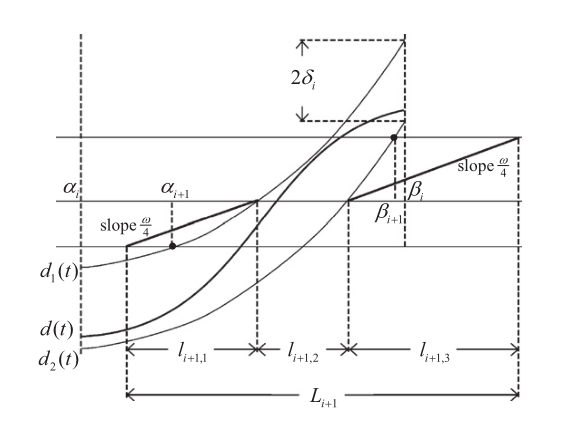
\includegraphics[width=0.7\linewidth]{1}
  \caption{Situacija v $i$-tem koraku algoritma.}
  \label{slika1}
  \end{center}
%  \end{figure}
\end{figure}